\documentclass[a4paper]{article}
\usepackage{titling}
\usepackage{authblk}
\usepackage{fancyhdr}
\usepackage[hyphens]{url}
\usepackage{hyperref}
\usepackage{rsc}
\usepackage{siunitx}
\usepackage{graphicx}
\usepackage{mhchem}
\usepackage{amsmath}
\usepackage{listings}
\usepackage{color}
\usepackage[htt]{hyphenat}
\usepackage{subcaption}

\definecolor{dkgreen}{rgb}{0,0.6,0}
\definecolor{gray}{rgb}{0.5,0.5,0.5}
\definecolor{mauve}{rgb}{0.58,0,0.82}
\graphicspath{{../figures/}}

\lstset{frame=tb,
  language=Python,
  aboveskip=3mm,
  belowskip=3mm,
  showstringspaces=false,
  columns=flexible,
  basicstyle={\ttfamily},
  numbers=none,
  numberstyle=\tiny\color{gray},
  keywordstyle=\color{blue},
  commentstyle=\color{dkgreen},
  stringstyle=\color{mauve},
  breaklines=true,
  breakatwhitespace=true,
  tabsize=3,
  postbreak=\mbox{\textcolor{red}{$\hookrightarrow$}\space}
}

\title{Lecture 8: Working with vectors and matrices}
\author[1]{Dr Benjamin J. Morgan}
\author[1,2]{Dr Andrew R. McCluskey}
\affil[1]{Department of Chemistry, University of Bath, email: b.j.morgan@bath.ac.uk}
\affil[2]{Diamond Light Source, email: andrew.mccluskey@diamond.ac.uk}
\setcounter{Maxaffil}{0}
\renewcommand\Affilfont{\itshape\small}
\newcommand{\bvec}[1]{\mathbf{#1}}
\newcommand{\norm}[1]{\left\lVert #1\right\rVert}
\newcommand{\cvec}[2]{\begin{bmatrix}#1\\#2\end{bmatrix}}

\pagestyle{fancy}
\fancyhf{}
\rhead{CH40208}
\lhead{\thetitle}
\rfoot{\thepage}

\begin{document}
\maketitle

\section*{Aim}
This week gives a brief introduction to \emph{vectors} and \emph{matrices}, and using these to perform mathematical manipulations in Python. 

Working with vectors and matrics is common in computational chemistry, and understanding the underlying mathematical concepts helps with understanding the algorithms that are used, and the code that implements them. Working with vectors and matrices falls within the branch of mathematics called \emph{linear algebra}. The next two weeks aim to give you a taste of some of the mathematical properties of vectors and matrics, and why using these can be useful in computationally solving chemical problems. 

If you would like to learn more about vectors, matrices, and linear algebra, I recommend the \emph{Essence of Linear Algebra} 3Blue1Brown YouTube series\footnote{\url{https://www.youtube.com/watch?v=fNk_zzaMoSs}}. Another useful resource is the \emph{Land on Vector Spaces} series of Jupyter notebooks by Lorena Barba's group\footnote{\url{https://github.com/engineersCode/EngComp4\_landlinear}}, which provides Jupyter-friendly tools for visualising vectors and matrix operations. If you prefer a more formal textbook, I recomment \emph{Introduction to Linear Algebra} by Gilbert Strang\footnote{\url{http://math.mit.edu/\~gs/linearalgebra/}}.

\section{Vectors}
Many problems in chemistry and physics involve working with \emph{vector} quantities. A common definition of a vector in a physics context is a quantity with both \emph{magnitude} and \emph{direction}; for example, the positions or velocities of atoms, or the forces acting on atoms within a molecule.

\subsection{Example 1: Atomic positions}
Defining atomic positions requires three pieces of information: the location of a reference position, called the \emph{origin}, the distance of each atom from the origin, and the direction we move from the origin to reach each atom. Positions are therefore \emph{vector} quantities (Fig.~\ref{fig:position_vectors}).
\begin{figure*}
  \centering
  \begin{subfigure}[t]{0.475\textwidth}
    \centering
    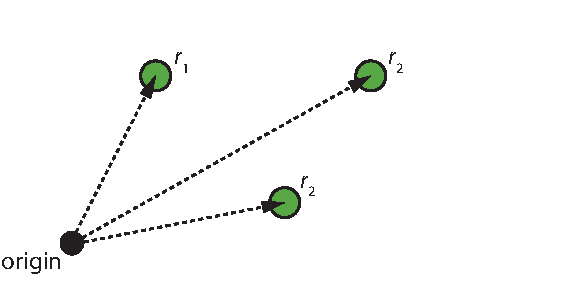
\includegraphics[width=\textwidth]{position_vectors_1}
    \caption[Network2]%
      {{\small Defining atomic positions requires knowing both distance and direction with respect to some reference \emph{origin}.}}    
    \label{fig:position_vectors_1}
  \end{subfigure}
  \hfill
  \begin{subfigure}[t]{0.475\textwidth}  
    \centering 
    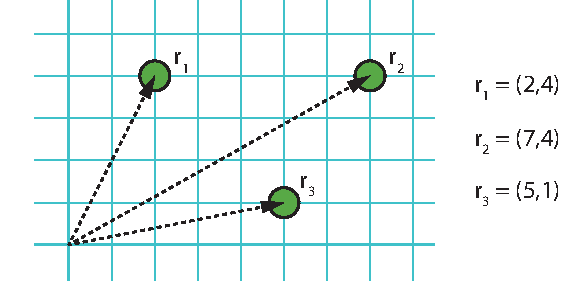
\includegraphics[width=\textwidth]{position_vectors_2}
  \caption[]%
      {{\small Describing positions using Cartesian coordinates, i.e.\ $(x,y)$ coordinates in two dimensions, or $(x,y,z)$ in three dimensions.}}    
    \label{fig:position_vectors_2}
  \end{subfigure}
  \vskip\baselineskip
  \begin{subfigure}[t]{0.475\textwidth}   
    \centering 
    \includegraphics[width=\textwidth]{position_vectors_3}
    \caption[]%
      {{\small The choice of coordinate system implicitly defines \emph{basis} vectors, $\bvec{i}$ and $\bvec{j}$. Any position can be expressed as a linear combination of these basis vectors.}}    
    \label{fig:position_vectors_3}
  \end{subfigure}
  \quad
  \begin{subfigure}[t]{0.475\textwidth}   
     \centering 
     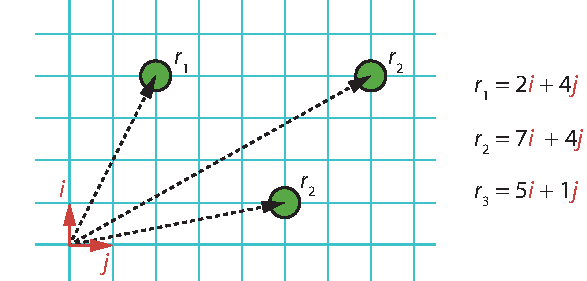
\includegraphics[width=\textwidth]{position_vectors_4}
     \caption[]%
       {{\small The $(x,y)$ coordinates given in \ref{fig:position_vectors_2} are the coefficients used to define each position in the basis $(\bvec{i},\bvec{j})$.}}    
     \label{fig:position_vectors_4}
   \end{subfigure}
 \caption
   {} 
 \label{fig:position_vectors}
\end{figure*}
A common choice for describing atomic positions is to use Cartesian coordinates, i.e.~$(x,y)$ in two dimensions, or $(x,y,z)$ in three dimensions \footnote{A good choice of coordinate system depends on the problem at hand, and Cartesian coordinated may not always be easiest to work with. For example, problems with spherical symmetry, such as describing atomic orbitals, will often be simpler when expressed in spherical coordinates $(r, \phi, \theta)$.}; this will be familiar from the interatomic distances (week 2) and molecular rotation (week 4) problems. In two dimensions, any position can be described by giving both the $x$ coordinate and the $y$ coordinate. Using the language of vectors, this choice of $x$ and $y$ coordinates defines a pair of \emph{basis} vectors, which we will denote $\bvec{i}$ and $\bvec{j}$ 
\footnote{Vectors are usually distinguished from scalar variables by using upright bold text, e.g.~$\bvec{r}$ (used here) or an accenting arrow, e.g.~$\vec{r}$. The components of a vector can be given as a list, e.g.~$(1,2)$, or as a column vector, e.g.~$\begin{bmatrix}1\\2\end{bmatrix}$. These two representations correspond to the same vector $1\vec{i}+2\vec{j}$.}. 
$\bvec{i}$ is a vector of length $1$ pointing along $x$ and $\bvec{j}$ is a vector of length $1$ pointing along $y$. Any position vector $\bvec{r}=(x,y)$ can be expressed as a \emph{linear combination} of these basis vectors, i.e.\ $\bvec{r} = x \times \bvec{i} + y \times \bvec{j}$. This means one way to think about the usual notation $(x,y)$ is that the two numbers describe the coefficients of $\bvec{i}$ and $\bvec{j}$ for a given linear combination. This might seem an overly complicated way of thinking about coordinates in Cartesian space, but it highlights that writing down a position vector such as $(3,4)$ is only meaningful if the basis vectors are defined. If we had chosen a different set of basis vectors, the \emph{same} positions would be described with \emph{different} vectors.
\begin{figure}[tb]
  \centering
  \resizebox{7cm}{!}{\includegraphics*{position_vectors_alternate_basis.pdf}} %
    \caption{\label{fig:position_vectors_alternate_basis}The three positions from Fig.~\ref{fig:position_vectors}, in a different basis.}
\end{figure}

\subsection{Vector addition, subtraction, scaling, and ``multiplication''}
Vectors can be added together by adding the coefficients of each basis vector (Fig.~\ref{fig:vector_addition}). For example, adding together the vectors $\bvec{v}_1=(5,1)$ and $\bvec{v}_2=(2,4)$ gives us a new vector $\bvec{v}_3=(7,6)$. \begin{figure}[htb]
  \centering
  \resizebox{7cm}{!}{\includegraphics*{vector_addition.pdf}} %
    \caption{\label{fig:vector_addition}Vector addition,.}
\end{figure}
This rule is explained by writing $\bvec{v}_1$ as $(5\bvec{i}+1\bvec{j})$ and $\bvec{v}_2$ as $(2\bvec{i}+4\bvec{j})$. Adding $\bvec{v1}$ and $\bvec{v2}$ then gives $\left[(5\bvec{i}+1\bvec{j})+(2\bvec{i}+4\bvec{j})\right]$ and common terms can be collected together to give $\left[(5+2)\bvec{i}+(1+4)\bvec{j}\right]=(7\bvec{i}+6\bvec{j})$. Subtracting one vector from another follows the same rules, but with the coefficients of each basis vector subtracted; e.g. $\bvec{v}_1-\bvec{v}_2=(3,-3)$. 

Scaling a vector involves multiplying by a \emph{scalar} (hence the name). This changes the length of the vector, but not the direction, and involves multiplying each of the basis vector coefficients by the scalar value. i.e.~$\bvec{v}_\mathrm{1}=(2,3)$. $\bvec{v}_1\times2=(4,6)$. Again, we can understand this by expanding out the original vector in terms of the basis vectors, $\bvec{i}$ and $\bvec{j}$: $(2\bvec{i}+3\bvec{j})\times2=(4\bvec{i}+6\bvec{j})$.

\subsubsection{The dot-product and the cross-product}
We can also ``multiply'' two vectors together, although this is more complex. In fact there are \emph{two} standard ways to define ``multiplication'' of vectors.

The \emph{dot product} is also known as the ``scalar product''. This operation takes two vectors and returns a scalar quantity. The dot product of two vectors is denoted $\bvec{a}\cdot\bvec{b}$, and is defined as
\begin{equation*}
\bvec{a}\cdot\bvec{b} = \sum_ia_ib_i = a_1b_1 + a_2b_2 + \ldots + a_nb_n.
\end{equation*}
For example, if $\bvec{a}=(2,1)$ and $\bvec{b}=(3,2)$ then $\bvec{a}\cdot\bvec{b}$ is given by
\begin{eqnarray*}
\bvec{a}\cdot\bvec{b} & = & (x_\mathrm{a} \times x_\mathrm{b})+ (y_\mathrm{a}\times y_\mathrm{b})\\
& = & (2\times3 + 1\times2) \\
& = & 8
\end{eqnarray*}
An equivalent definition of the dot product is
\begin{equation*}
\bvec{a}\cdot\bvec{b} = \norm{\bvec{a}}\norm{\bvec{b}}\cos\theta,
\end{equation*}
where $\norm{\bvec{a}}$ is the \emph{length} of vector $\bvec{a}$, and $\theta$ is the angle between $\bvec{a}$ and $\bvec{b}$.

The \emph{cross-product} is also known as the ``vector product''. This operation takes two vectors and returns a vector quantity, with both magnitude and direction. The cross product between vectors $\bvec{a}$ and $\bvec{b}$ is denoted $\bvec{a}\times\bvec{b}$ and is defined as a vector \emph{perpendicular} to the plane containing $\bvec{a}$ and $\bvec{b}$ with a length given by the parallelogram with $\bvec{a}$ and $\bvec{b}$ as sides (Fig.~\ref{fig:cross_product}). 
\begin{figure}[tb]
  \centering
  \resizebox{11cm}{!}{\includegraphics*{cross_product.pdf}} %
    \caption{\label{fig:cross_product}The cross product of $\bvec{a}$ and $\bvec{b}$ is proportional to the area $A$ of the parallelogram with sides $\bvec{a}$ and $\bvec{b}$.}
\end{figure}
This can be computed as
\begin{equation*}
\bvec{a}\times\bvec{b} = \norm{\bvec{a}}\norm{\bvec{b}}\sin\theta\,\bvec{n},
\end{equation*}
where $\bvec{n}$ is the \emph{unit vector} (a vector with length 1) perpendicular to the plane containing $\bvec{a}$ and $\bvec{b}$.

\section{Working with vectors in Python}
Working with vectors in Python is made simple by using \texttt{numpy} arrays.
\begin{lstlisting}
import numpy as np

# define two 2D vectors using numpy arrays
>>> a = np.array([5,1])
>>> b = np.array([2,4])
>>> print(a)
[5, 1]
>>> print(b)
[2, 4]

# vector addition
>>> c = a + b
>>> print(c)
[6, 5]

# vector subtraction
>>> d = a - b
>>> print(d)
[3, -3]
\end{lstlisting}
Remember that multiplication of \texttt{numpy} arrays involves element-wise multiplication and returns a new array.
\begin{lstlisting}
# vector multiplication?
>>> e = a * b
>>> print(e)
[10, 4]
\end{lstlisting}
This is \emph{not} the same as $\bvec{a}\cdot\bvec{b}$ or $\bvec{a}\times\bvec{b}$. Instead we can use the \texttt{numpy.dot()} and \texttt{numpy.cross()} functions:
\begin{lstlisting}
# dot product
>>> dot = np.dot(a,b)
>>> print(dot)
14

# cross product
>>> cross = np.cross(a,b)
>>> print(cross)
18
\end{lstlisting}

\vspace{\baselineskip}
\begin{center}
  \noindent\fbox{%
      \begin{minipage}{0.9\textwidth}%
          \vspace{0.15\baselineskip}
      \subsubsection*{Exercise}
          In week 2 you wrote some code to calculate interatomic distances (and angles) between pairs of atoms in example molecules, using the expression
          \begin{equation*}
          r_{ij} = \sqrt{(x_i-x_j)^2+(y_i-y_j)^2+(z_i-z_j)^2}.
          \end{equation*}
          Starting from your week 2 code, or from scratch, write a new version of this code that solves the problem using \texttt{numpy} arrays and \texttt{np.dot}.

          The \texttt{molecule1.txt} and \texttt{molecule2.txt} files can be downloaded from Moodle.
      \end{minipage}
  }
\end{center}

\section{Matrices as linear transformations}

We saw previously that the elements of a vector can be thought of as the coefficients in a linear combination of basis vectors, i.e.~ $\begin{bmatrix}a\\b\end{bmatrix}=(a, b)=a\times\bvec{i}+b\times\bvec{j}$. This means that a specific vector is only meaninful if the corresponding basis is defined. A suitable choice of basis vectors depends on the problem we are interested in solving, and there are many situations where it can be useful to change from one set of basis vectors to another: for example a molecular dynamics simulation might use atomic positions, velocities, and accelerations in Cartesian coordinates, corresponding to a Cartesian basis, and usually called the \emph{lab} frame of reference. The dynamics of individual molecules, however, might be easier to describe within a \emph{molecular} frame of reference, with basis vectors aligned with specific bonds or along rotational axes. In this case, modelling our system involves \emph{transforming} between these two sets of basis vectors.

As an example consider Fig.~\ref{fig:rotation_example}. This shows an initial  basis with $\bvec{i}=\cvec{1}{0}$ and $\bvec{j}=\cvec{0}{1}$, and a vector $\bvec{r}$:
\begin{equation*}
\bvec{r}=\cvec{3}{4}=3\bvec{i}+4\bvec{j}. 
\end{equation*}
We now rotate our basis by $\ang{90}$ anti-clockwise, which gives us a new vector $\bvec{r^\prime}$, which has elements $(3,4)$ in this new, rotated, basis;
\begin{equation*}
\bvec{r^\prime}=\cvec{3}{4}^\prime=3\bvec{i^\prime}+4\bvec{j^\prime},
\end{equation*}
where a prime symbol indicates we are in the new basis.
\begin{figure}[tb]
  \centering
  \resizebox{12cm}{!}{\includegraphics*{rotation_example.pdf}} %
    \caption{\label{fig:rotation_example}An example of a linear transformation: rotation by \ang{90} anticlockwise.}
\end{figure}
What is the vector $\bvec{r^\prime}$ in the \emph{old} basis? We can see from Fig.~\ref{fig:rotation_example} that this should be $(-4,3)$, but can we calculate this?

We start by expressing the \emph{new} basis vectors, $\bvec{i^\prime}$ and $\bvec{j^\prime}$, in terms of the \emph{old} basis vectors, $\bvec{i}$ and $\bvec{j}$:
\begin{equation*}
\bvec{i^\prime} = (0\bvec{i}+1\bvec{j}) = \cvec{0}{1};
\end{equation*}
\begin{equation*}
\bvec{j^\prime} = (-1\bvec{i}+0\bvec{j}) = \cvec{-1}{0}.
\end{equation*}
We can now expand the vector $\bvec{r^\prime}$ in terms of $\bvec{i}$ and $\bvec{j}$:
\begin{eqnarray*}
\bvec{r^\prime}&=&(3\bvec{i^\prime}+4\bvec{j^\prime})\\
               &=&3(0\bvec{i}+1\bvec{j})+4(-1\bvec{i}+0\bvec{j})\\
               &=&-4\bvec{i}+3\bvec{j}.
\end{eqnarray*}
We can also write this as a single \emph{matrix} equation, where we multiply each element of our original vector $\bvec{r}$ by the corresponding \emph{column} of our matrix,
\begin{equation*}
\bvec{r^\prime} = \begin{bmatrix}0 & -1 \\ 1 & 0\end{bmatrix}\bvec{r}.
\end{equation*}
which looks like
\begin{eqnarray*}
\begin{bmatrix}0 & -1 \\ 1 & 0\end{bmatrix}\cvec{3}{4} & = & 3\cvec{0}{1}+4\cvec{-1}{0} \\
  & = & \cvec{0}{3} + \cvec{-4}{0} \\
  & = & \cvec{-4}{3}.
\end{eqnarray*}
If we denote our matrix as $\bvec{M}$, this can be written concisely as
\begin{equation*}
\bvec{r^\prime} = \bvec{M}\,\bvec{r}.
\end{equation*}
\subsection{Inverse matrix operations}
We now have a matrix that describes a \ang{90} anti-clockwise rotation. What if we want to \emph{invert} this rotation, and rotate by \ang{90} in a clockwise direction? If we follow the same procedure as above, we end up with a matrix $\bvec{N}=\begin{bmatrix}0 & 1\\ -1 & 0\end{bmatrix}$, where
\begin{equation*}
\bvec{r} = \bvec{N}\,\bvec{r^\prime}.
\end{equation*}
The matrix $\bvec{N}$ is called the \emph{inverse} of the matrix $\bvec{M}$.
\subsection{Matrix--matrix multiplication}
What happens if we perform two matrix operations, one after the other? For example we perform \emph{two} successive \ang{90} rotations---giving a \ang{180} rotation?

Mathematically this looks like
\begin{eqnarray*}
\bvec{r^{\prime\prime}}&=&\bvec{M}\,\bvec{r^\prime} \\
& = & \bvec{M}\left(\bvec{M}\,\bvec{r}\right) \\
& = & \bvec{M}\,\bvec{M}\,\bvec{r}.
\end{eqnarray*}
We first operate on $\bvec{r}$ with $M$, to get $\bvec{r^\prime}$, and then operate on this vector again with $\bvec{M}$. What is the result of this double operation, and can find a matrix that describes a general rotation by \ang{180}?

Written out, $\bvec{M}\,\bvec{M}$ looks like
\begin{equation*}
\bvec{M}\,\bvec{M}= \begin{bmatrix}0 & -1\\ 1 & 0\end{bmatrix}\begin{bmatrix}0 & -1\\ 1 & 0\end{bmatrix}.
\end{equation*}
We can determine the corresponsing matrix for a \ang{180} rotation by considering what happens to the basis vectors $\bvec{i}$ and $\bvec{j}$ when we operate on them twice with $\bvec{M}$.
\begin{eqnarray*}
\begin{bmatrix}0 & -1\\ 1 & 0\end{bmatrix}\begin{bmatrix}0 & -1\\ 1 & 0\end{bmatrix}\bvec{i} = \begin{bmatrix}0 & -1\\ 1 & 0\end{bmatrix}\begin{bmatrix}0 & -1\\ 1 & 0\end{bmatrix}\cvec{1}{0}
\end{eqnarray*}
As we saw above, the first operation (working from right to left) converts $\bvec{i}$ to $\bvec{i^\prime}=\cvec{0}{1}$. We now calculate the effect of the second operation
\begin{equation*}
\begin{bmatrix}0 & -1\\ 1 & 0\end{bmatrix}\cvec{0}{1} = 0\cvec{0}{1} + 1\cvec{-1}{0} = \cvec{-1}{0}.
\end{equation*}
Doing the same for $\bvec{j^\prime}$ gives
\begin{equation*}
\begin{bmatrix}0 & -1\\ 1 & 0\end{bmatrix}\cvec{-1}{0} = -1\cvec{0}{1} + 0\cvec{-1}{0} = \cvec{0}{-1}.
\end{equation*}
And we remember that the columns of a matrix describe the new basis functions, in this case $\bvec{i^{\prime\prime}}$ and $\bvec{j^{\prime\prime}}$. The matrix that describes a \ang{180} rotation (or two successive \ang{90} rotations) is therefore $\begin{bmatrix}-1 & 0\\ 0 & -1\end{bmatrix}$, i.e. both $x$ and $y$ are inverted.

\section{Matrices in Python}
Matrices can be described by multidimensional \texttt{numpy} arrays, and we can perform matrix multiplication with the \texttt{numpy.matmul()} function\footnote{You can get the same results using \texttt{numpy.dot()}, but we encourage \texttt{numpy.matmul()} because it makes the final code easier to read and follow.}.
\begin{lstlisting}
>>> r = np.array(3,4)
>>> M = np.array([[0,-1],
                  [1, 0]])
>>> r_prime = np.matmul(M,r)
>>> print(r_prime)
[-4 3]
\end{lstlisting}
The inverse of a matrix can be calculated (if it exists) using \texttt{numpy.linalg.inv()}.
\begin{lstlisting}
>>> N = np.linalg.inv(M)
>>> print(N)
[[ 0.  1.]
 [-1. -0.]]
>>> np.matmul(N, r_prime)
[3, 4]
\end{lstlisting}
Matrix--matrix multiplication can also be performed with \texttt{numpy.matmul()}:
\begin{lstlisting}
>>> MM = np.matmul(M,M)
>>> print(MM)
[[-1  0]
 [ 0 -1]]
 \end{lstlisting}


\vspace{\baselineskip}
\begin{center}
  \noindent\fbox{%
      \begin{minipage}{0.9\textwidth}%
          \vspace{0.15\baselineskip}
      \subsubsection*{Exercise}
          In week 4 you wrote some code to rotate a molecule in two-dimensions. The equations for the rotation of coordinates $(x,y)$ by $\beta$ are 
          \begin{eqnarray*}
          x^\prime & =&  x \cos \beta - y \sin \beta \\
          y^\prime & = & y \cos \beta + x \sin \beta.
          \end{eqnarray*}
          By considering the effect of this rotation on the basis vectors $\bvec{i}$ and $\bvec{j}$ derive the rotation matrix for a rotation around the origin by $\beta$.

          Starting from your previous code, or from scratch, create a module named \texttt{matrix\_transform} that includes a function \texttt{rotation}. that will take three variables \texttt{x}, \texttt{y}, and \texttt{angle}. This function will perform a rotation of \texttt{angle} on \texttt{x} and \texttt{y} to produce \texttt{x\_new} and \texttt{y\_new}, which are returned from the function. Use the \texttt{visualisation.show()} function to observe the rotation of the water molecule.

          The \texttt{water.txt} file and the \texttt{visualisation.py} module can be downloaded from Moodle.
      \end{minipage}
    }
\end{center}
%\bibliographystyle{rsc}
%\bibliography{handout_5}

\end{document}
